%----------------------------------------------------------------------------
\chapter{Jegyzőkönyv}
%----------------------------------------------------------------------------

%----------------------------------------------------------------------------
\section{Megvalósított függvények}
%----------------------------------------------------------------------------
A képfeldolgozás a processImage függvényben történik, melyet a keretprogram minden új képkockára meghív. A képfeldolgozást megvalósító függvényeket kellett itt meghívni. 
\begin{itemize}
	\item \textbf{getRoi} - A \textit{Region of Interest} (ROI) kivágása az eredeti képből a \textit{Bounding Box} (BB) alapján, melyet az inicializálás során egérrel határozzuk meg, később a program frissíti
	\item \textbf{getDepthMask} - A függvény megkeresi a ROI terület közepét, és elmenti az ahhoz a képponthoz tartozó mélység értéket. Leellenőrzi, hogy nem történt-e hirtelen ugrás az előző értékhez képest, ha ez nem következett be, akkor az azonos távolságú pixelek alapján maszkot készítünk, mellyel visszatér a függvény.
	\item \textbf{getHueMask} - A könnyebb képfeldolgozás érdekében HSV színtérbe konvertáljuk a ROI által meghatározott képrészletet, majd az első lefutáskor meghatározzuk a benne leggyakrabban szereplő színt, melyet a \textit{getMaxHue} függvénnyel valósítunk meg. Színszűréssel készítünk egy második maszkot. A fekete és a szürke pixeleket kizárjuk, mivel ezek \textit{Hue} értéke bizonytalan.
	\item \textbf{getMaxHue} - Hisztogramot készítünk a kapott kép pixeleinek \textit{Hue} értékéből, amennyiben azok nem szürkék vagy feketék. A függvény a leggyakrabban előforduló színértékkel tér vissza.
	\item \textbf{getLargestMask} - A függvény a bemenetként megadott bináris maszkban kontúrokat keres és a legnagyobb területű kontúrt és az ezáltal meghatározott objektum momentumait adja vissza. Mi ezt a távolság és szín érték alapján meghatározott maszkok metszetével hívtuk meg.
	\item \textbf{compute3D} - A megtalált objektum térbeli pozícióját számolja ki, az előtte már meghatározott \textit{Center of Gravity} (COG) és a kép paraméterei alapján. 
	\item Ezen megvalósított függvények mellett a \textit{processImage}-ben a COG és a BB frissítésre kerül. 

\end{itemize}
A megvalósított program a következő kimenetet eredményezte:
KÉP, SOK KÉP

\begin{figure}[!h]
	\centering
	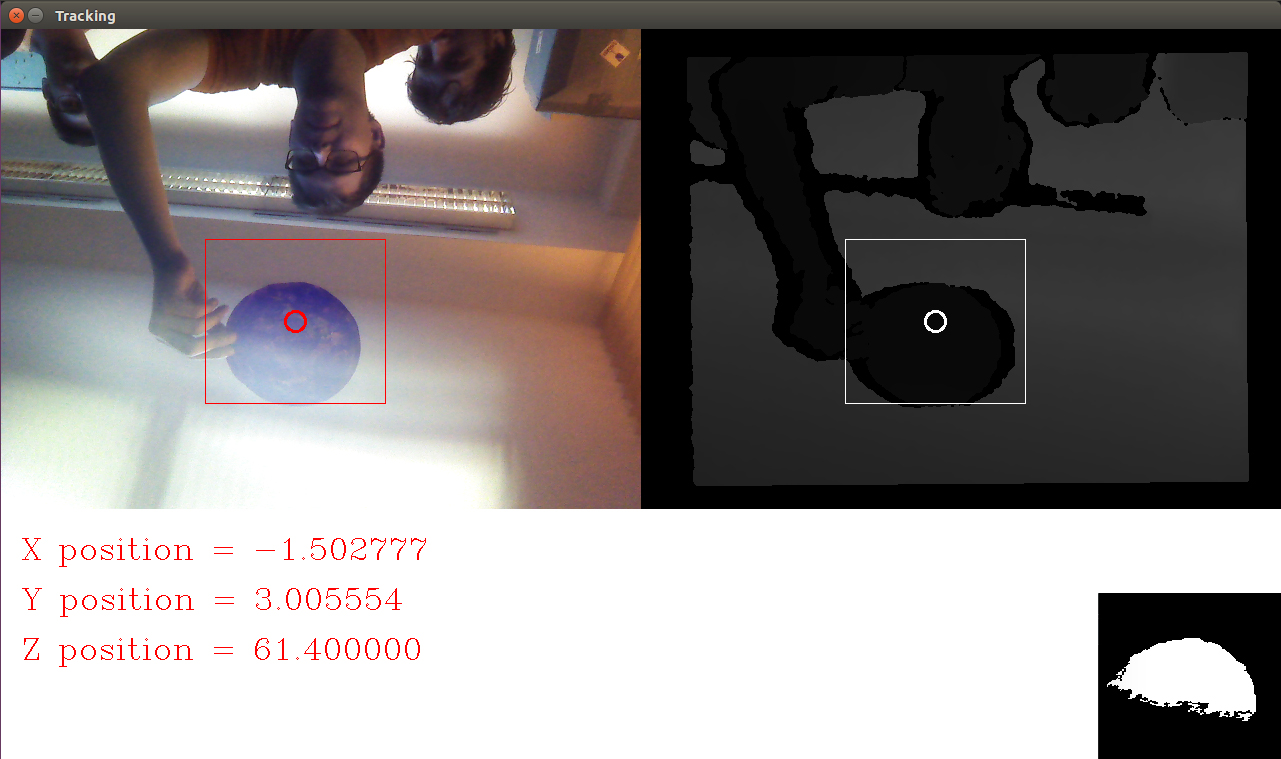
\includegraphics[width=69mm, keepaspectratio]{figures/m08/fig1.jpg}\hspace{5mm}
	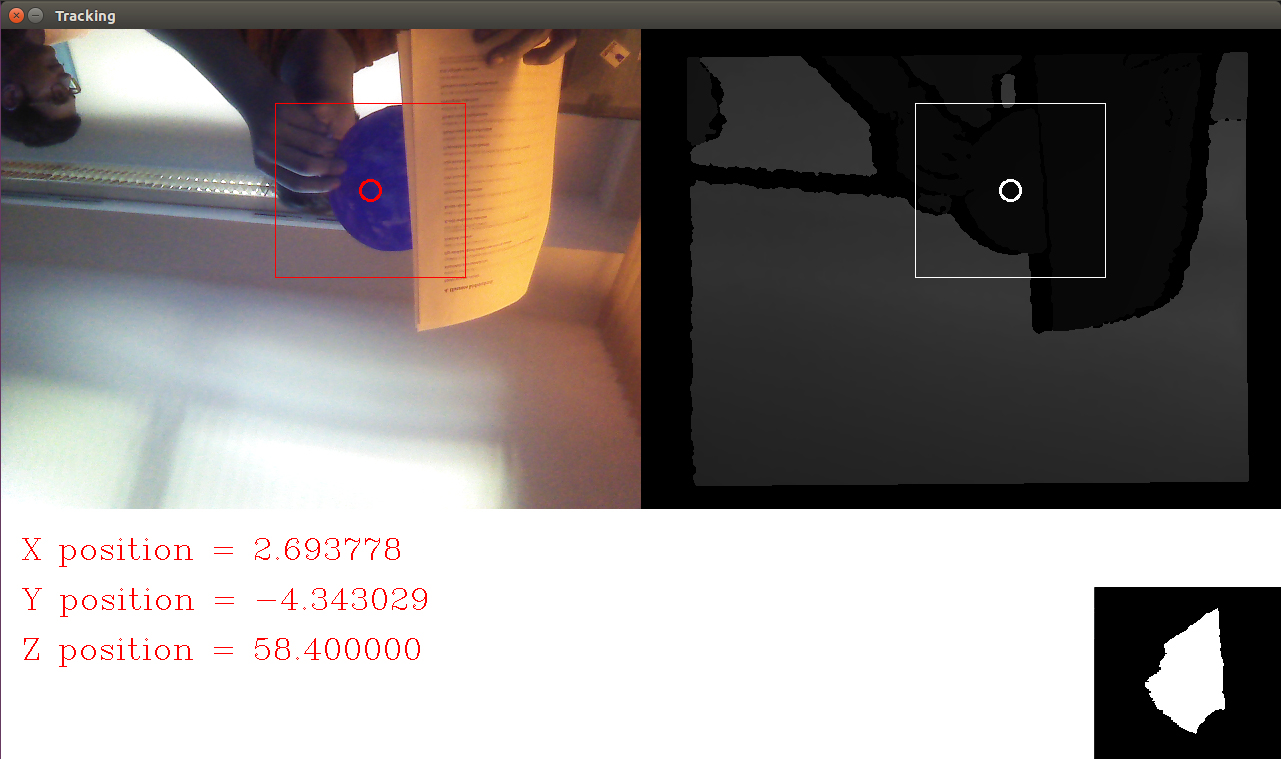
\includegraphics[width=69mm, keepaspectratio]{figures/m08/fig2.jpg}\\\vspace{5mm}
	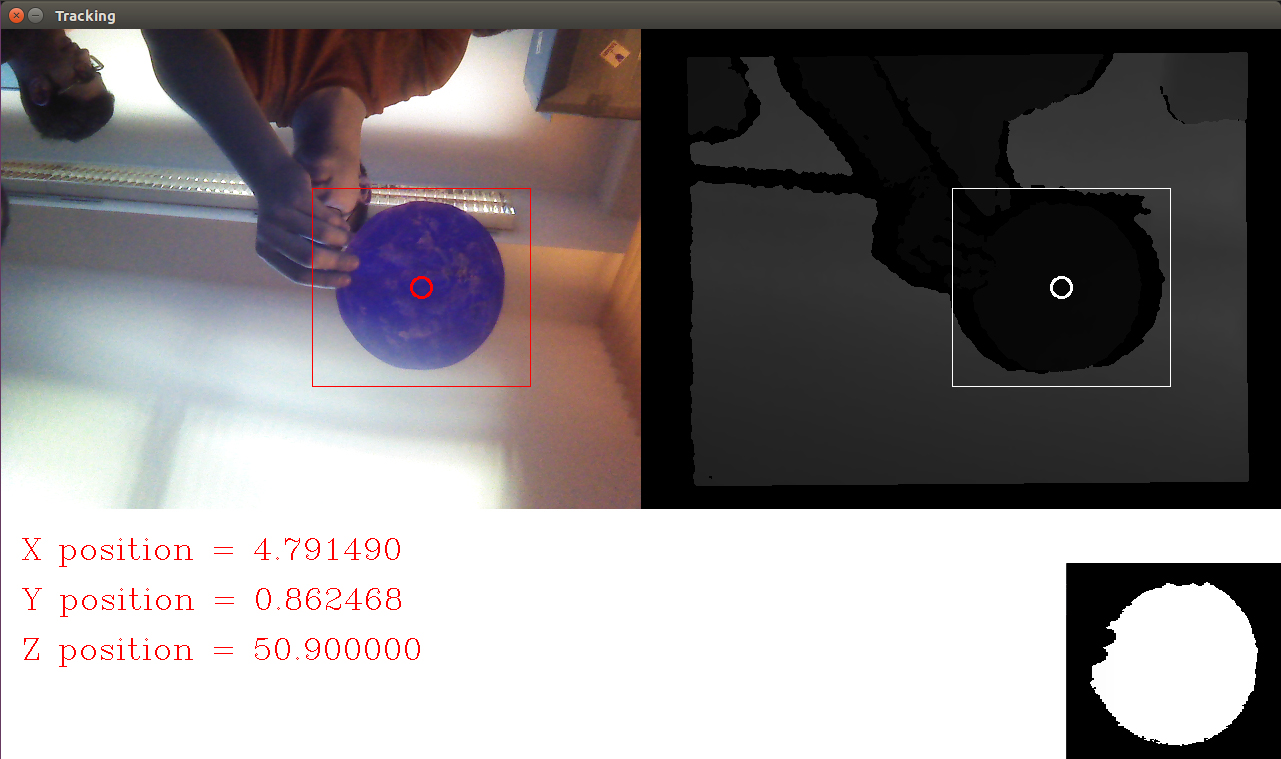
\includegraphics[width=69mm, keepaspectratio]{figures/m08/fig3.jpg}\hspace{5mm}
	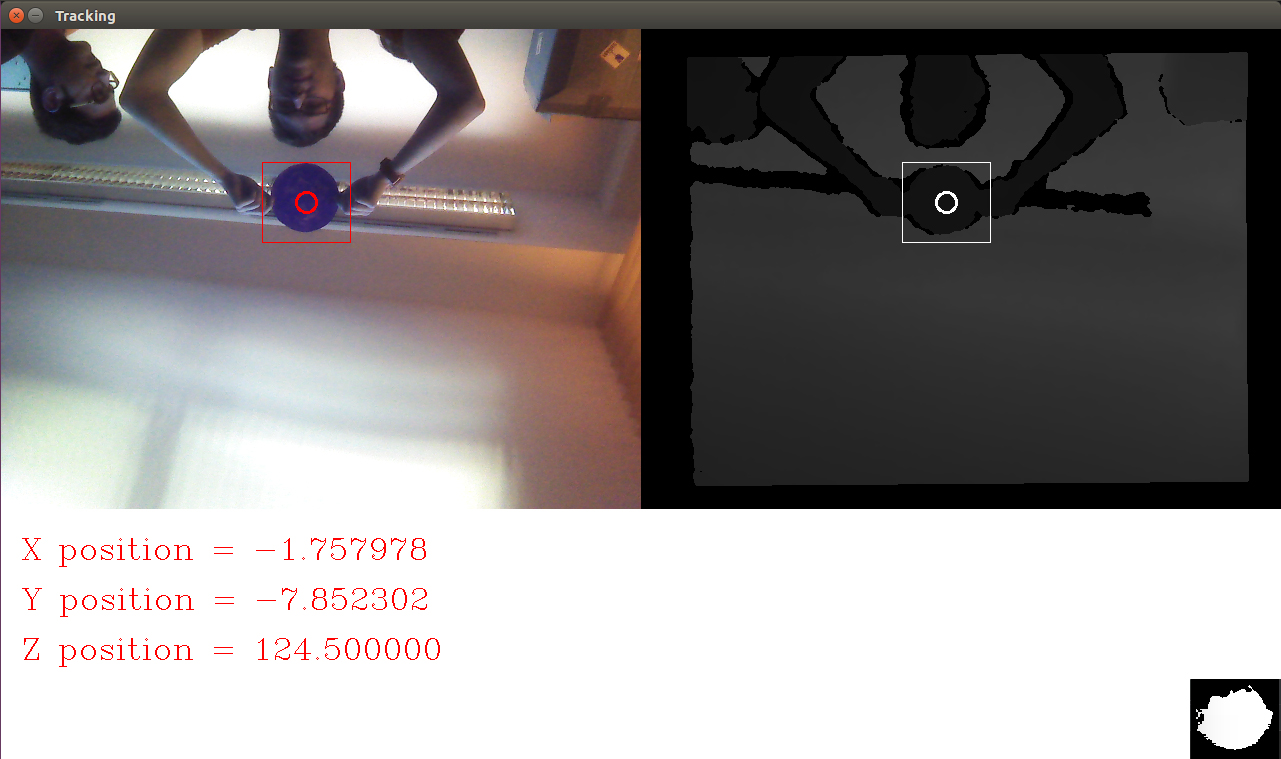
\includegraphics[width=69mm, keepaspectratio]{figures/m08/fig4.jpg}
	\caption{A megvalósított objektumkövetés, az aktuális maszkokkal} 
	\label{fig:Dejong}
\end{figure}

%----------------------------------------------------------------------------
\section{Konklúzió}
%----------------------------------------------------------------------------
\begin{itemize}
	\item Az \textbf{OpenCV} a képeket BGR alakban kezeli a sok helyen megszokott RGB helyett, mely miatt a keresendő piros objektum a Hue skálán 120 körüli értéket vesz fel a 0 helyett. Így a szűrt tartomány 100 és 140 közé esik a 160-20 helyett, mely egyszerűbben implementálható.
	\item Kezdetben a feladat elején csak a \textit{Depth} maszkot használtuk, mellyel az objektum követés már megvalósítható volt, ám a maszk készítésnél a belógó tárgyak, pl a kezünk torzította az objektumot. Továbbá az inicializált objektum elé helyezett tárggyal átverhetővé vált a program, immár az új tárgyra valósult meg az objektumkövetés. Ez a szín szűréssel lényegesen javítható.
	\item Mivel bármilyen \textit{Hue} érték esetén, ha a \textit{Value} 0 fekete színt kapunk, így a fekete pixelek szín szerinti szűrése véletlen eredményt okozna, mely zajt hozna a rendszerbe. A kis szaturációjú (szürke)  színek szintén ezt okoznák, emiatt ezeket is szűrjük.

\end{itemize}







